\chapter{Artifact}

In this chapter, the system's context and it's dependencies as well as the architecture, some interesting features, used technologies and conducted testing are presented. Design decisions, implementation alternatives and resulting consequences are introduced and discussed along the lines.

\section{System Context}

The reimbursement-tool interacts with several user types as well as external software systems. In this section, these actors and software systems are introduced and existing dependencies outlined.

\subsection{Actors}

The context diagram as shown in figure \ref{fig:context-diagram} describes the relationships between the system and its users:
\textit{Expense Creators}, such as assistants, professors and other employees can create, view and print expenses. However, they are only allowed to modify their own expenses while these are in the draft state i.e have not been submitted to the \textit{Expense Creator}'s manager yet.  \textit{Managers}, such as professors, the department manager, the head of institute and the finance administration personnel are able to \textit{reject expenses} and send them back to the expense creators. Besides rejecting expenses, they are also able to modify them. Moreover, \textit{Managers} have also to provide for each expense a project description. \textit{Finance administrators} can additionally to the \textit{managers} aggregate statistics, search for certain expenses, re-assign expenses that are stuck in the process (e.g. when a manager would have to sign the expense but left the IFI) and reset expenses that have been rejected by the finance administration UZH. \textit{Guests} are allowed to view specific expenses and related expense-items too. However, they need the 32-character long internal expense \textit{Uid} to gain access to the expense's details. The \textit{Uid} is added on the printed expense document (see appendix \ref{sec:app-pdf}).

\begin{figure}[H]
	\centering
	\fbox{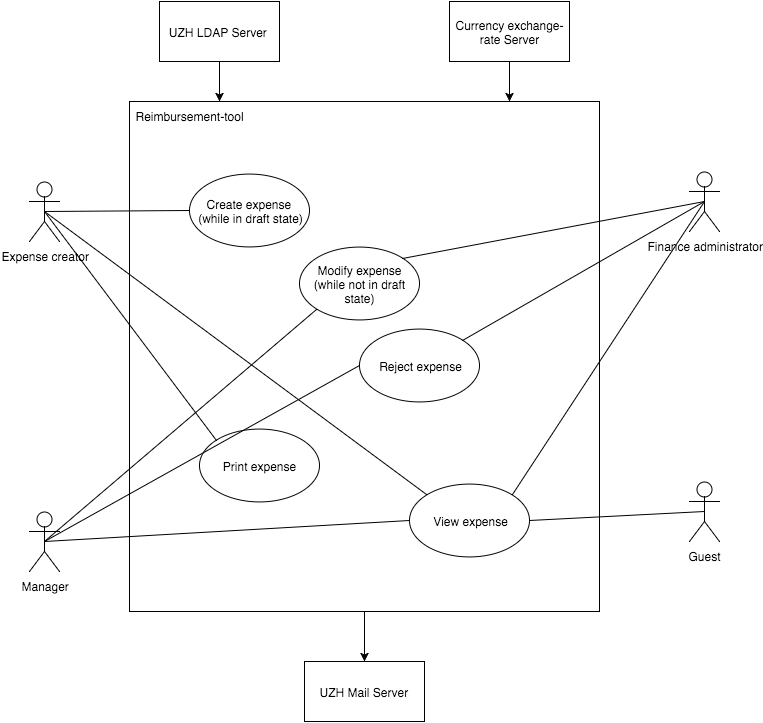
\includegraphics[width=1\textwidth]{context-diagram}}
	\caption{System context: Context diagram}
	\label{fig:context-diagram}
\end{figure}

\subsection{Services and Dependencies}
The following sub sections explain what external systems are required to operate the reimbursement tool (please also refer to figure \ref{fig:context-diagram}).

\subsubsection{IFI LDAP Server}
The reimbursement-tool fetches user-data from the IFI LDAP server  and stores it in the reimbursement-database.  For more information about the features that require this dependency please refer to \ref{feature:ldap}. For details about how to adjust the LDAP settings to \ref{subsubsec:ldap}.

\subsubsection{Currency Exchange-Rate Service}
To handle currency conversions in an efficient way, we decided to use \textit{fixer.io}\cite{fixer}. \textit{Fixer.io} is free, updated daily, provides low response times and a high availability. While the \textit{European Central Bank(ECB)}\cite{ecb} is used as data source in the background, \textit{fixer.io} provides a query-able web-service for the ECB's data. More about the integrated currency feature in \ref{feature:currency}.

\subsubsection{IFI Mail Server}
\label{dep:email}
To notify users about actions that need their attention, the reimbursement-tool implements a notification algorithm. As soon as a new action has to be taken, the notification service generates an email and sends it to the related user. More about the notification feature in \ref{feature:notification}. The reimbursement tool integrates the IFI Mail Server for the actual sending of the e-mails. For more information about adjusting the e-mail settings please refer to \ref{subsubsec:e-mail}.


\section{Special Features}

\subsection{E-mail Notifications}
\label{feature:notification}

\subsubsection{Description}
To inform the users of the reimbursement-tool about expense state changes or other issues that require the user's attention, e-mail notifications have been implemented.
E-mail notifications are sent out in the following situations:
\begin{itemize}
	\item An expense, that has been created by a \textit{Expense Creator}, is assigned to a \textit{Manager}. An e-mail will be sent to the respective \textit{Manager}.
	\item An expense that has been approved by the \textit{Manager} and enters the state \newline \textbf{TO\_BE\_ASSIGNED}. This will trigger an e-mail to all available users with role \textit{Finance administration}.
	\item An expense that needs to go through the signing process. The next user in the row will get an e-mail. First the \textit{Expense Creator}, then it's \textit{Manager} and finally the assigned person from the \textit{Finance administration}.
	\item If an expense is rejected by a \textit{Manager} or the \textit{Finance administration} the \textit{Expense Creator} of the expense will receive an e-mail notification.
\end{itemize}

As soon as a new action has to be taken, the notification service adds the user's e-mail address to the e-mailing list. E-mails are sent out as often as specified in the configuration (currently 8am, 12pm and 5pm). At this points in time, the e-mailing list is processed by checking if there are still actions (also from the past) that need the user's attention. If that is the case, an e-mail is sent out. If in the meantime the user took the required action, no e-mail is sent out. If after an e-mail sending no new action occurs, no reminder-e-mail will be sent although there are remaining actions. For the actual e-mail sending, the reimbursement-tool integrates the IFI Email Server (as depicted in \ref{dep:email}).

Besides the above mentioned state changes, e-mails are also sent out to warn the administrator of the reimbursement-tool of major incidents and if general run-time exceptions occur.

\subsubsection{E-mail Settings and Configuration}
\label{subsubsec:e-mail}

The e-mail settings can be adjusted in the \\ \texttt{application.properties} file in the back-end. To change the layout of an email, the corresponding email template has to be altered. The email templates are stored in the directory \textit{src/main/resources/email}. To adjust an email template, we recommend to change the non-inlined version (\textit{src/main/resources/email/notInlinedTemplates}) and then inline it by using an inlining service like \textit{Ink.} (\url{http://foundation.zurb.com/emails/inliner.html}). To change the wording of the emails, the source texts in the "EmergencyEmailSendJob.java" and "NotificationSendJob.java" classes have to be adapted. These files are stored on the back-end in \textit{/src/main/java/ch/uzh/csg/reimbursement/model} folder. \newline \\
Some of the variables in the \texttt{application.properties} file depend on the Maven profile and are therefore specified in the \texttt{pom.xml} file that is stored in the back-end's root folder.

\begin{lstlisting}[numbers=left, breaklines=true]
# If true this option stores an HTML
# file on the server instead of sending it to the email-receiver.
# the exact location can be seen in the email-log.
mail.redirectMailsToFile = ${mail.redirectMailsToFile}

# This cron trigger defines when the email are sent out
# http://www.quartz-scheduler.org)
mail.sendEmailsIntervalCron = ${mail.sendEmailsIntervalCron}
\end{lstlisting}


\subsection{LDAP Synchronisation}
\subsubsection{Description}
\label{feature:ldap}
\textbf{User friendliness: }By being able to reuse the existing LDAP credentials, the user gets a comfortable way to login and ensures at the same time that only authenticated users gain access to the system.\par 
\textbf{User Management: }The reimbursement-tool fetches user-data from the IFI LDAP server and stores it in the reimbursement-database. The user's current roles and the user's manager are then assigned automatically.  If there is no manager specified in the LDAP, a warning is shown to the user. As a whole, this is a convenience feature facilitating the user management.

\subsubsection{LDAP Settings and Configuration}
\label{subsubsec:ldap}

Currently the synchronisation interval is set to 300 seconds. This value can be changed by adjusting the variable \textit{reimbursement.ldap.refreshRate} in the \texttt{application.properties} file that is stored in the back-end at \textit{src/main/resources} \par
During the development and integration a specific file will be loaded that defines the available demo user-accounts for the reimbursement-tool. Those users are defined in the file \texttt{development-server.ldif}. The following users exist:
\begin{itemize}
	\item \texttt{junior} is a representative for the \textit{Junior Assistants} group defined in the IFI LDAP tree.
	\item \texttt{senior} is a representative for the \textit{Senior Assistants} group defined in the IFI LDAP tree.
	\item \texttt{prof} is a representative for the \textit{Professors} group defined in the IFI LDAP tree.
	\item \texttt{fadmin} \& \texttt{fadmin2} are representatives for the \textit{Administration} group defined in the IFI LDAP tree.
	\item \texttt{Depman} is a representative for the \textit{Departement Manager} defined in the IFI LDAP tree.
	\item \texttt{Headinst} is a representative for the \textit{Head of Institute} defined in the IFI LDAP tree.
	
\end{itemize}

For all the demo user-accounts, the password is \textit{password}. To be able to login with the demo users, the test-ldap server has to run (is automatically started if the build profile is "DEV" or "INT") and also the demo-user SQL has to update the SQL Database (also done automatically in the "DEV" or "INT" profiles). Please refer to the Maven Profiles' \ref{sub:profiles} section for further information.

\subsection{PDF Generation}
\subsubsection{Description}
The PDF Generation feature enables a conversion of images to Pdf and also the final transformation of the data gathered in the process into the required PDF Document.

\subsubsection{PDF Generation Implementation Details}
\label{subsubsec:pdf-xml-mappings}

The \textit{.xsl} file is used to generate an \textit{.fo} file out of an xml-file that consists of object data. In the folder \textit{src/main/resources} exists a \texttt{xml-mapping.xml} file that maps a data-object to a xml-object. The xml-object is required by the \texttt{xml2fo.xsl} and \texttt{attachmentXml2fo.xsl}. Those files transfer the xml-object into a \textit{.fo} file which is needed by the Apache FOP to generate the Pdf.

\subsection{Integrated Currency Conversion}
\label{feature:currency}
Often expenses accrue in foreign currencies but are paid back in CHF. To provide the user with a handy but still accurate way to calculate the historically accurate amount that has to be charged back, the reimbursement tool integrates a currency-exchange-rate-service. Currently, the reimbursement-tool calls the API every time an exchange-rate is needed. For example if the user specifies the amount of a receipt in a foreign currency. Since the API is called by our reimbursement-server, any cheating regarding exchange rates is prevented.


\subsection{Signature Registration: mobile enabled}
Instead of uploading an image showing their manual signature, we integrated a signature-pad. This pad allows the user to register its signature by using a touch-enabled device. This makes the registration process much easier: instead of signing on paper, scanning or photographing the paper, removing the background and uploading it, the users can simply sign on their smartphone, tablet or other touch-enabled device. This features makes use of tokens that expire after a certain timeout. This timeout can be specified in the \textit{applications.properties} file.

\subsection{Attachment Upload: mobile enabled}
To allow an efficient way to create expense receipts, we implemented the possibility to photograph the receipts with ones smartphone or other camera-enabled device. This makes the general reimbursement-creation process much faster, since everything can be done without leaving one's desk. Scanned documents are of course still supported. This features makes use of tokens that expire after a certain timeout. This timeout can be specified in the \textit{applications.properties} file.

\subsection{Signing of Documents}
The ability to sign the printed Pdf document is crucial so that authenticity is guaranteed. Especially if the Pdf document will be used as evidence by the Finance Administration of the University of Zurich. The system provides two types of signatures \cite{arx-signature}:
\begin{itemize}
	\item A \textbf{Digital signature} ensure the authenticity of the signer. Any changes made to the document after it has been signed will invalidate the signature. To use it the user has to provide his private key to successfully sign the document.
	\item \textbf{Electronic signature} does \textbf{not} ensure the authenticity of the signer. Anyone can theoretically make changes on the document after it has been signed without the signature become invalid. Of course, in our tool this is prevented by design. The handwritten signature captured during the registration will be stamped on the Pdf document.
\end{itemize}\par

\textbf{Pure offline signing: }Due to the requirement, that the private key cannot be uploaded or processed by the server, the digital signing needs to be done on the client using a modern web-browser. The implementation of the digital signature is therefore done using a third party library called \textit{pdfsign.js}\cite{pdfsign}. \textit{Pdfsign.js}  is further presented in section \ref{tec:pdfsign}.\par

\subsection{Guest View}
The reimbursement-tool provides the "Guest View". The guest view is a view especially designed and implemented to allow an anonymous user (e.g the Finance Administration of the University of Zurich) to view a dedicated expense with related expense items and all other information. The access to the information is granted for users that know the 32-character long internal expense \textit{Uid}. The \textit{Uid} is added on the printed expense document. To see an example, please refer to appendix \ref{sec:app-pdf}.\par 

This features makes use of tokens that expire after a certain timeout. This timeout can be specified in the \textit{applications.properties} file.


\subsection{Multi-language capability}
The reimbursement-tool supports an easy extension of additional languages. Currently, "English" and "German" are available. To add another language on the client, only the \textit{/reimbursement-client/src/languages/languages.json} has to be extended with the translations and the navigation-bar extended with the additional language option. \newline 
On the server, translations for the e-mail texts have to be added. Please refer for further information to the e-mail section in \ref{subsubsec:e-mail}.

\subsection{CORS and CSRF support}
In development the back-end runs on Tomcat and the front-end on Node.js, the two applications do not share the same domain (differing port). This causes the browsers "same origin policy" to prevent the loading of data. We solved this issue by implementing CORS. CORS offers several benefits compare to JSONP and is the de-facto standard approach to solve this issues. \par 

To also allow a similar architecture in a productive environment, though not needed at the moment, we also implemented "Cross Site Request Forgery" prevention.

\subsection{Deputy Feature}
Good workers need and also deserve holidays. In order to allow expenses to be managed while someone is on holiday, the system automatically forwards the required activities like validation or signing to the deputy. For every employee, its deputy is assigned based on the information stored in LDAP.

\subsection{Expense Pool}
At the Finance Administration of the IFI more then one employee takes care for the expenses in the expense reimbursement process. The \textit{expense pool} is a container for all expenses that were submitted to IFI's finance administration personnel. Every finance administrator can self-assign these expenses and validate or reject them. After a finance administrator has assigned an expense to him/her, the expense will for signing be directly assigned to the same administrator.

\subsection{Cost Category Management}
Every expense has to be assigned to a cost category but \textit{Expense Creators} have hard time figuring out which cost category is the right one. The reimbursement-tool supports the\textit{ Expense Creators }by showing a detailed description in the user's language. The \textit{finance administration} can at any time add or disable cost-categories in the respective administration screen. If users have expenses that are assigned to a disabled cost-category, the next time they edit the cost-category they are prompted to chose another cost-category.

\subsection{Basic Statistics Feature}
For the Finance Administration of IFI, some basic visualizations for the different states of the employees, as well as the total amount of open reimbursement cash-backs have been integrated in the user interface.

\subsection{Expense Search Engine}
To make the Finance Aadministrations work more productive, a search engine support the search for open and archived expenses. This search is especially usful in combination with the reset feature.

\subsection{Expense Reset Options}
\textbf{Stuck-in-process:} The expense reset feature allows the \textit{Finance Administration IFI} to reset expenses, that are stuck in the process. This can happen if an employee has an inactive manager without deputy that should sign an expense. The employee has to contact the finance administration IFI. In this case, one of \textit{Finance Administrators} can reset the expense and a default reject-message, nicely written in the \textit{expense creator}'s language, will be shown as reject reason. Before restarting, the new manager has to be assigned in the LDAP. \par

\textbf{Rejected-by-UZH:} While in the first case the reason for the rejection is obvious and expected by the \textit{Expense Creator}, the reason if the finance administration UZH rejects an expense is more complex. To inform the \textit{Expense Creator} about the reason, the \textit{Finance Administrator} at IFI has the possibility to enter a custom rejection message. Either the \textit{Finance Administrator} can edit the expense and the process continues with the signing by the \textit{Expense Creator}, or the expense has to be edited by the \textit{Expense Creator} and the process restarts with the validation steps.

\subsection{Archiving}
All users can archive printed expenses. This removes the expenses from the dashboard and shows them in a separate part of the user interface. Like this, the dashboard which is optimized for the day-to-day work remains clear, neat and does not get cluttered by already processed expenses.

\newpage
\section{Architecture}

The back-end consists of a web-application running on a Tomcat \cite{tomcat} server and a PostgreSQL\cite{postgresql} database. The infrastructure is hosted and maintained by the IFI. The front-end/client communicates with the back-end using a RESTful service interface described in section \ref{sec:restfulapi}.

\subsection{Multilayered Architecture}
We decided to use a common \textit{Multilayered architecture (MLA)}\cite{mla} (see figure \ref{fig:architecture-layer}). The main design principle behind MLA is the Separation of Concerns (SoC), that enforces a division of code with different responsibilities in distinct parts. In consequence, the software is well structured and remains maintainable also over time. The following four layers are essential:
\begin{itemize}
	\item The \textbf{Data Access Layer} consists of repositories and the \textit{Hybernate} database abstraction. Depending on the build-profile, different database types are used. The Data Access Layer hides the resulting complexity and provides a uniform interface for storing and retrieving data to and from the database.
	\item The \textbf{Business Layer} provides the business logic available as services to the \textit{Application Layer}. It performs all business relevant modifications on the models by using the \textit{Data Access Layer}.	
	\item The \textbf{Application Layer} provides a uniform RESTful API that can be used by any client. This may be a web-application, an app or another server. It hosts the Security part, the REST resources and the Global Exceptions Handlers.
	\item The \textbf{Presentation Layer} provides the front-end code. In our case it uses AngularJS for the GUI creation. The \textit{Presentation Layer} interacts with the \textit{Application Layer} by accessing its RESTful API using asynchronous Javascript and JSON.
\end{itemize}

\begin{figure}[H]
	\centering
	\fbox{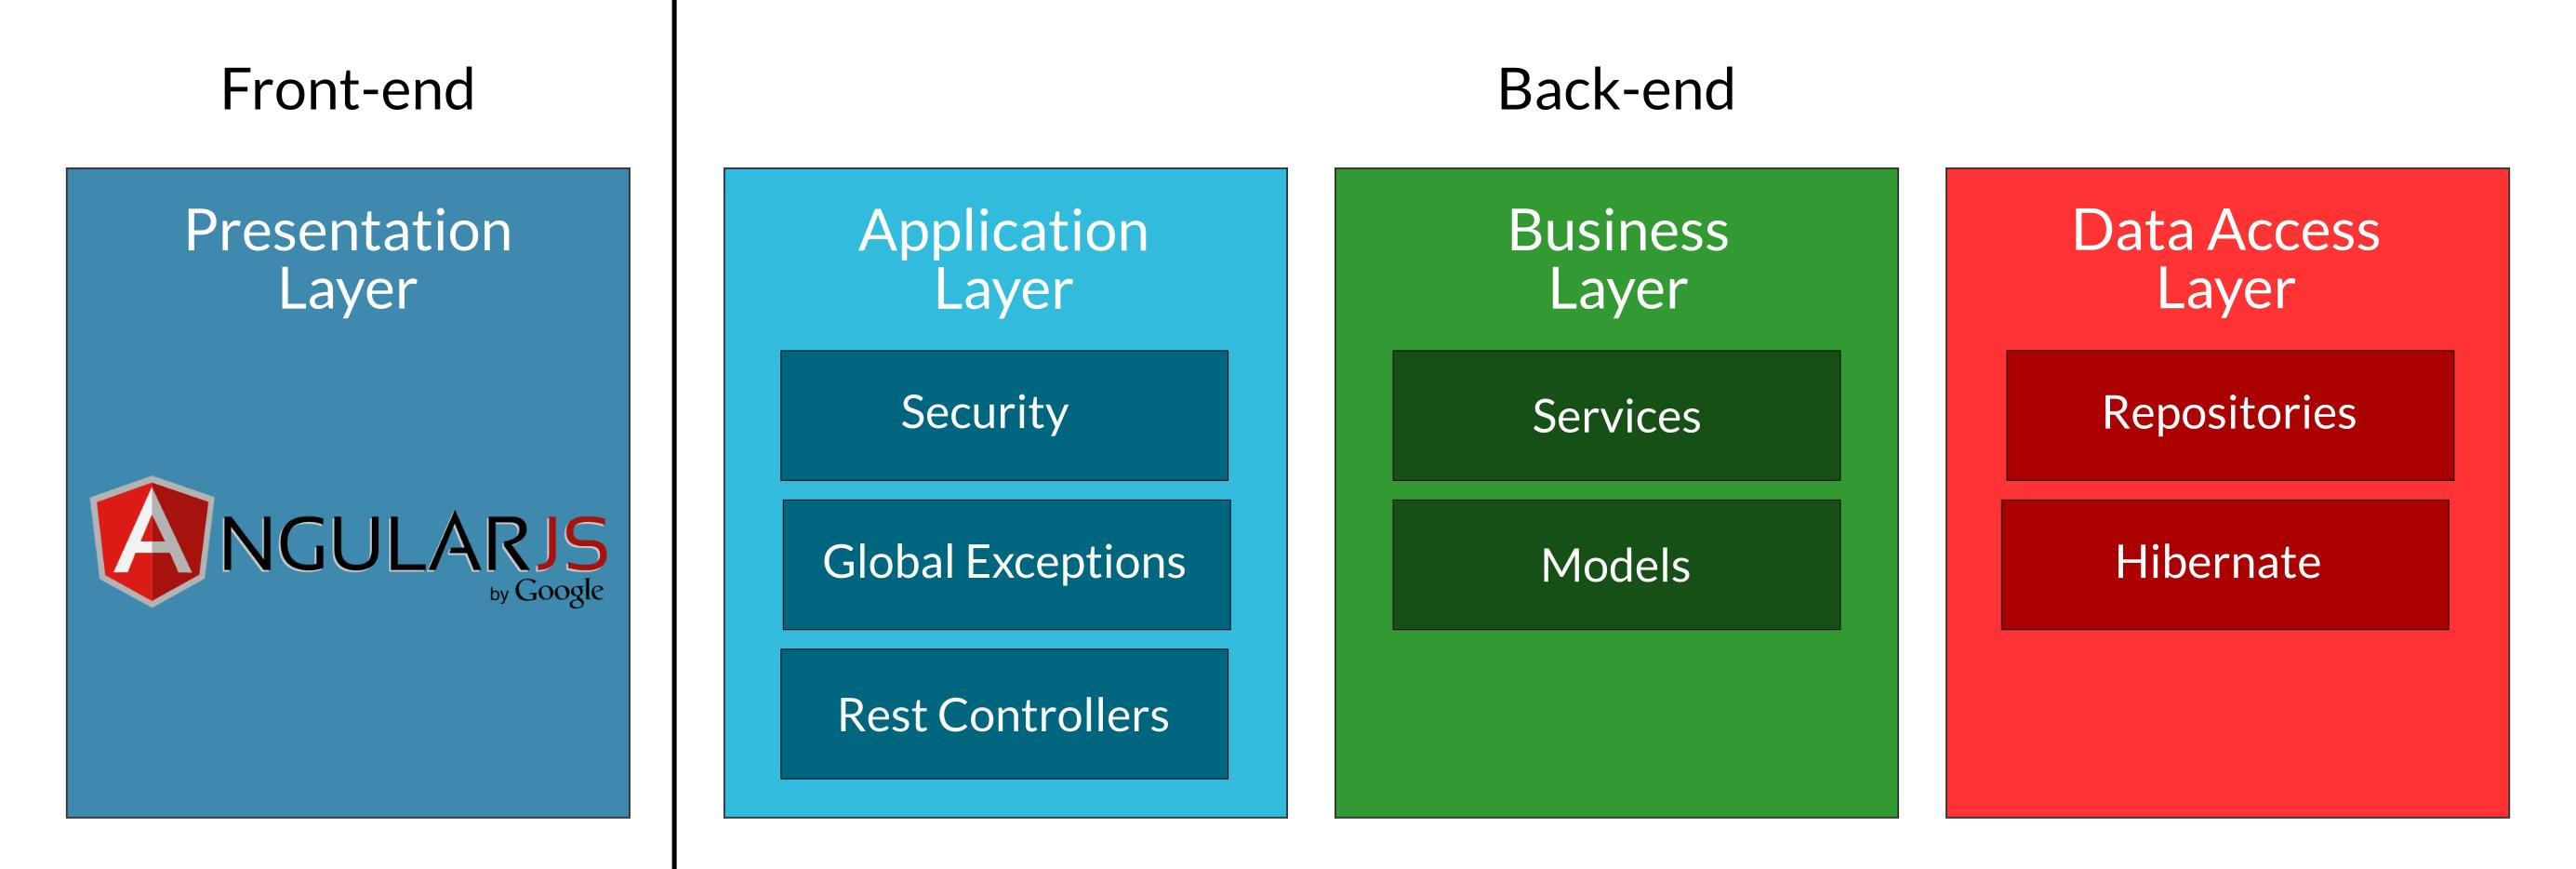
\includegraphics[width=0.80\textwidth]{architecture-layer}}
	\caption{Architecture: Multilayer architecture}
	\label{fig:architecture-layer}
\end{figure}

Our layers depend on each other while every layer communicates only with either the upper (consumer) or the lower (service provider) layer. This ensures a good maintainability and loose coupling of the single layers.\newline
At this point an example should be given: If the \textit{presentation layer} needs to display an expense, the \textit{application layer} will handle this request by first checking the relevant security parameter of the request followed by calling the \textit{business layer}. The \textit{business layer} will handle and aggregate the desired information fetched from the relevant models. In our case to display an expense, the service will retrieve all expense-items and expense-item-attachments from the database using the \textit{data access layer}. Since the \textit{data access layer} provides a uniform interface, the \textit{business layer} does not care if a H2 or Postgres database is used - it just calls the interface and gets the information. The \textit{business layer} passes the data to the \textit{application layer}, where it is serializes as JSON and sent as request-response to the \textit{presentation layer}. There, the data is processed and displayed in the GUI.

\subsection{Back-end}
The back-end is structured according to the rules of a multilayered software architecture. We use the domain driven design \cite{ddd} to apply common patterns for the different layers. The domain model, that consists of the concepts, is connected to the database. Changes on the model will be automatically synchronized with the database. The service package lists all methods that are used on a domain model.\newline
Data Transfer Objects (DTO) are used to transfers data from back-end to front-end and vice verse. \newline 
The implemented model- and service-classes are visualized in appendix \ref{sec:app-models} and \ref{sec:app-service}.

\subsection{Front-end}
The front-end is developed in JavaScript using the AngularJS framework\cite{angular}. AngularJS is based on a MVC (Model View Controller) pattern. It basically consists of controllers, templates that are used for the view  as well as models representing the data that is shown to the user using the templates. However, AngularJS  extends the basic MVC concept with useful enhancements like directives, filters, injectors etc. A complete list of the available concepts in AngularJS can be found in the AngularJS Developer Guide \cite{angular-devguide}.

\subsection{RESTful API}
\label{sec:restfulapi}
The tool uses a RESTful API that provides services to access the back-end resources. It is implemented using the Spring Framework, which is introduced in the next chapter. \newline 
The available methods provided by the back-end are listed in \ref{sec:rest-services}. There exist private and public services. Private services can only be access by a \textbf{Registered user / User} (private services are marked with the term PRIVATE).

\section{Technologies}

In the following section the technologies used are described and explained why they were chosen.

\subsection{Back-end}

\subsubsection{Java}
The reimbursement-tool uses for the back-end part Java SE 7. Java is a mature programming language developed and maintained by Oracle\cite{java}, has detailed documentation and since Java is taught at IFI's Info 1 course, an adequate support and further development of the reimbursement tool can be guaranteed.

\subsubsection{Hibernate}
\textit{Hibernate} abstracts the data layer. So that SQL-queries have to be written in rare cases only, which increases the code-clarity and decreases the code-complexity. All data operation are handled implicitly by defined Java data classes.\newline
H2 database is a temporary database for storing data in a database environment. It offers a simple interface and can be used for development, given that only one development database server is available. \cite{hibernate}

\subsubsection{Spring Framework}
We decided to use the \textit{Spring Framework}\cite{spring} because it's well documented, widely used and easy to integrate in an existing Java project. We use various components and sub-packages of Spring. These are:
\begin{itemize}
	\item Spring Security for the login- and user-management as well as role based access-management for the RESTful resources.
	\item Spring Web MVC is used to define RESTful interface within a few lines of code.
	\item Spring ORM used for the XML mapping within the process of Pdf-generation.
	\item Spring Data is used to provide a simpler method to use data access technologies. It uses the DAO (Data Access Object) \cite{dao} to access data in a standard database like SQL.
	\item Spring Test and Spring Security Test provide means for a convenient integration testing.
\end{itemize}

\subsubsection{Maven}
The tool uses Apache Maven\cite{maven} for the build process and dependency management. We decided to use it, because it is widely used and is easy to maintain with a single \textit{pom.xml} file.

\subsubsection{Apache FOP}
The generated Pdf by the reimbursement-tool needs to be identical to the existing MS Excel file provided by the Finance Administration of the University of Zurich. The generated Pdf structure is added in \ref{sec:app-pdf}.\newline
The Pdf gets generated using an individually created XSLT template while the XML document is generated out of a Java Object. Combining these two files generates an \textit{.fo} document, which will be used by Apache FOP \cite{apache-fop} to generate the Pdf.\par
We favoured Apache FOP because it is based on widely used standards like XML and XSL. This ensures further maintenance.

\subsubsection{Pdfsign.js}
\label{tec:pdfsign}
\textit{PDFSign.js} is a JavaScript library that signs a PDF in the browser. \textbf{No} private keys or passwords are ever sent over the network. The signing takes place in the browser only. The signing part is done with an adapted version of \textbf{forge}. The PDF parsing is done with a stripped down version of \textbf{PDF.js}. For more information about this library, please consult the \textit{PDFSigns} Github project \cite{pdfsign} straight. 

\subsubsection{Swagger UI}

The Swagger UI visualizes all methods provided by the RESTful interface using a simple GUI. Furthermore developers can interact directly with the Swagger UI to test the \texttt{HTTP} methods. Figure \ref{fig:swagger01} shows a screen-shot of our Swagger UI. It visualizes all the available methods for the \texttt{public} resource as well as the mandatory and optional parameters for \texttt{HTTP} calls. This was important for the process of development. \cite{swagger} \par
We decided on Swagger UI, because a simple and easy to understand overview, as well as a simple integration into the software source-code. Further testing the back-end functionality was very simple using Swagger UI.

\begin{figure}[H]
	\centering
	\fbox{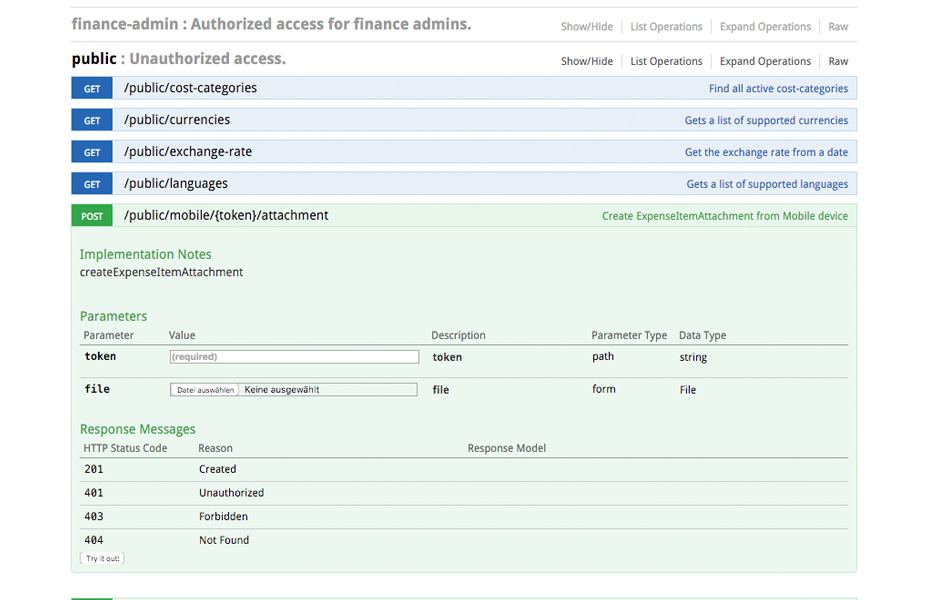
\includegraphics[width=0.80\textwidth]{swagger01}}
	\caption{Swagger: Reimbursement GUI}
	\label{fig:swagger01}
\end{figure}

\subsection{Front-end}

\subsubsection{AngularJS}
The tool uses the AngularJS framework. Its data bindings and dependency injections reduces the amount of code need to be written. Further it uses HTML templates and an sophisticated routing concept to deliver interactive GUIs. AngularJS is based on an MVC approach and is easy to integrate with REST services.\cite{angular}\par
We used AngularJS because of its broad community and the fact that it's supported by Google makes it future-proof.

\subsubsection{Bootstrap}
Bootstrap is a framework that consists of HTML, CSS and JavaScript elements. It can be used to create appealing responsive websites. Further it's CSS elements are supported by most of the desktop and mobile web-browsers available. The tool uses Bootstrap v. 3.3.5. \cite{bootstrap}\par
We use Bootstrap to speed-up the GUI development process. Using the elements it provides makes it easy to setup a responsive website within minutes. Further it provides a lot of fancy HTML/CSS elements like \textit{accordions}, \textit{modals}, etc.

\subsubsection{Bower}
The tool uses Bower for the client-side package management. Bower is a package manager for JavaScript web applications like AngularJS. It keeps track of the used assets, frameworks, libraries, etc. \cite{bower} \par
We used Bower because of its widely used, has a sound documentation and is easy to work with.

\subsubsection{Grunt}
Grunt is a JavaScript task runner. We use it for our client-side build. Its plugin directory supports a lot of modules to optimize the development work flow. Code-uglifying, concatenating, sass-compiling, file operations, auto prefixing etc. \cite{grunt} \par
We used Grunt because its widely used and there exists sound know how about its usage in our team.



\section{Testing}

\subsection{Unit Testing}
Since the application is quite big in scope, the unit testing has in accordance with the supervisors been neglected. To still ensure a high software quality, integration tests are preferred.

\subsection{Integration Testing}
To detect the impact of code changes, integration tests cover the main scenarios. These are:
\begin{itemize}
	\item Registration
	\item Login
	\item Expense Creation
	\item Expense Item Creation
	\item Attachment upload
	\item Assigning of expenses to IFI Finadmins
	\item Validation of Expenses (Managers and IFI Finadmins)
	\item Digitally Signing
	\item End-To-End Process for Assistant-Prof-Finadmin-Assistant-Prof-Finadmin
	\item End-To-End Process for Prof-Finadmin-Prof-Depman-Finadmin
	\item End-To-End Process for Finadmin-Finadmin2-Finadmin-Depman-Finadmin2
	\item End-To-End Process for Depman-Finadmin-Depman-Headinst-Finadmin
	\item End-To-End Process for Headinst-Finadmin-Headinst-Depman-Finadmin
\end{itemize}


\subsection{Load Testing}
The reimbursement tool has been load-tested using the tools JMeter\cite{jmeter} in combination with VisualVM\cite{visualvm}.

\paragraph{Apache JMeter} "JMeter is an open source software designed to load test functional behavior and measure performance. It was originally designed for testing Web Applications but has since expanded to other test functions."\cite{jmeter}.\par

In JMeter, all required steps to perform a document upload have been modelled and compiled into a testsuite.

\paragraph{VisualVM} "VisualVM is a visual tool integrating several command line JDK tools and lightweight profiling capabilities. Designed for both production and development time use, it further enhances the capability of monitoring and performance analysis for the Java SE platform."\cite{visualvm}.\par 
\textit{VisualVM} enables the live monitoring of the active configuration, heap space, classes, instances and tasks running on the VM, where the application is deployed. For information regarding the monitoring of a remote host, please refer to the appendix \ref{appendix:visualvm} \par

\paragraph{Findings}
The load tests have shown, that the conversion of large images could cause a bottleneck. Since the image-formats are converted to PDF only on the back-end, large images consume a huge amount of the available heap. With 2gb heap space, only 6 parallel uploads of 8mb large images can be handled. A possible work-around would be to convert the images already on the client to pdf-format and only send the pdf-documents to the server.\par

Another potential bottleneck could arise if large amounts of expenses are in the dashboard. In this case, the back-end would serialize all data required to display these expenses in a single request. This could be mitigated by implementing \textit{pagination} i.e.expenses are sent to the client in chunks of size N. If more expenses are required, the back-end sends the second page, namely the second chunk of N expenses.

\subsection{User and GUI Testing}
The graphical user interface is simple and practical. Nevertheless it provides a good user guidance and pleases the eye with subtle animations.\par

The user interface of the front-end has been tested through the supervisors and Claudia Leibundgut and has been improved over numerous iterations. Since no business logic is present in the front-end, and the back-end handles all security relevant concerns, the programmatical testing of the front-end has been neglected.
